\section{黑洞}
\label{blackhole}
由于伪黎曼流形上的黎曼曲率是完全由度量决定的, 我们解爱因斯坦场方程实际上是想要解出一个度量. 有时候我们解出来的 $g_{\alpha\beta}$ 存在{\bf 奇点}, 这些奇点和所谓的{\bf 黑洞}密切相关.

对于 $(M,g_{\alpha\beta})$ 上的向量场 $\xi^{\alpha}$, 若 $\xi^{\alpha}$ 生成的单参微分同胚群中的微分同胚都是等距的, 则称 $\xi^{\alpha}$ 为 {\bf Killing 向量场}.

若 $(M,g_{\alpha\beta})$ 上存在类时 Killing 向量场, 则称 $(M,g_{\alpha\beta})$ 为{\bf 稳态时空}(stationary spacetime), 称 $g_{\alpha\beta}$ 为{\bf 稳态度量}. 

\begin{remark}
	稳态时空对应于引力场不随时间变化的情况 (\cite[\S\,8.1]{梁灿彬2000微分几何入门与广义相对论}).
\end{remark}

对于 $(M,g_{\alpha\beta})$ 上的向量场 $v^{\alpha}$, 若任取 $p\in M$ 都存在过点 $p$ 且与 $v^{\alpha}$ 处处正交的超曲面, 则称 $v^{\alpha}$ 是{\bf 超曲面正交的}(hypersurface orthogonal).

若 $(M,g_{\alpha\beta})$ 上存在超曲面正交的类时 Killing 向量场, 则称 $(M,g_{\alpha\beta})$ 为{\bf 静态时空}(static spacetime), 并称 $g_{\alpha\beta}$ 为{\bf 静态度量}.

对于稳 (静) 态时空, 其定义中的 Killing 向量场 $\xi^{\alpha}$ 的积分曲线所对应的参考系叫做 {\bf 稳(静)态参考系}, 其中的观者叫做 {\bf 稳(静)态观者}.

称 $(M,g_{\alpha\beta})$ 上的所有到自身的等距微分同胚构成的群为{\bf 等距微分同胚群}. 若 $(M,g_{\alpha\beta})$ 的等距微分同胚群含有一个与 $\mathrm{SO}(3)$ 同构的子群 $G_3$, 且 $G_3$ 的所有轨道都是 $2$ 维球面, 则称 $(M,g_{\alpha\beta})$ 为{\bf 球对称时空}(spherically symmetric spacetime).

\subsection{史瓦西真空解}
\begin{itemize}
	\item $1914$ 年, 一战爆发后, 史瓦西自愿加入德军, 时年 $41$ 岁.
	\item $1915$ 年 $11$ 月, 爱因斯坦提出广义相对论. 不久后, 史瓦西在俄罗斯战场前线给出了爱因斯坦场方程的第一个解析解 (史瓦西真空解), 并于同年 $12$ 月写信给爱因斯坦的告知他这一解法, 史瓦西在信中说道 ``As you see, the war treated me kindly enough, in spite of the heavy gunfire, to allow me to get away from it all and take this walk in the land of your ideas." 同年, 史瓦西患上了天疱疮.
	\item $1916$ 年 $3$ 月, 史瓦西退伍回国, 并于两个月后死于天疱疮.
\end{itemize}

假设宇宙中放着一个小球, 除此之外空无一物. 假设小球既不自转也不带电, 我们接下来计算这样的小球如何扭曲它外部的时空.

\begin{remark}
	我们接下来试图在 $\mathbb{R}^4$ 中解爱因斯坦方程.
\end{remark}

为了方便讨论, 我们使用线元记号来表示度量 (\S\,\ref{line element}), 即
\[ \mathrm{d}s^2=g_{\alpha\beta}\,\mathrm{d}x^{\alpha}\mathrm{d}x^{\beta}. \]

由于我们假设小球不自转, 应当假设时空是稳态的; 而为了得到时空的一个坐标系, 则进一步假设时空是静态的. 于是 $(M,g_{\alpha\beta})$ 上存在超曲面正交的类时 Killing 向量场 $\xi^{\alpha}$, 任取一个与 $\xi^{\alpha}$ 处处正交的超曲面 $\Sigma_0$, 任取 $\Sigma_0$ 上一个 (局部) 坐标系 $\{x^1,x^2,x^3\}$, 则通过 $\xi^{\alpha}$ 的积分曲线可以得到整个时空的坐标系 $\{t,x^i\}$, 具体方法为:
\begin{enumerate}
	\item 令 $\Sigma_0$ 上所有点的第一个坐标分量都是 $t=0$.
	\item 以积分曲线的参数 $t$ 作为曲线上每一点的第一个坐标分量.
	\item 以积分曲线与 $\Sigma_0$ 的交点的坐标 $(x^1,x^2,x^3)$ 作为曲线上每一点的其余三个分量.
\end{enumerate}
我们称这样的坐标系为{\bf 静态坐标系}, 并称所有第一个坐标分量为 $t$ 的点所构成的集合为该坐标系的{\bf 同时面} (simultaneity surface), 记作 $\Sigma_t$. 由构造知 $\Sigma_t$ 与 $\xi^{\alpha}$ 处处正交, 进而有
\[ g_{0i}=g_{\alpha\beta}\left( \frac{\partial }{\partial t} \right)^{\alpha}\left( \frac{\partial }{\partial x^i} \right)^{\beta}=0, \] 
因此可将线元表达为
\[ \mathrm{d}s^2=g_{00}(x^1,x^2,x^3)\,\mathrm{d}t^2+g_{ij}(x^1,x^2,x^3)\,\mathrm{d}x^i\mathrm{d}x^j. \] 

由于我们考虑的是仅存在一个小球的宇宙, 很自然地可以假设时空是球对称的. 考虑到 $(\mathbb{R}^3,\delta_{ij})$ 的线元
\[ \mathrm{d}s^2=\mathrm{d}x^2+\mathrm{d}y^2+\mathrm{d}z^2 \] 
在球坐标系
\[ \begin{aligned}
	x &= r\sin\theta\cos\varphi,\\
	y &= r\sin\theta\sin\varphi,\\
	z &= r\cos\theta,
\end{aligned} \]
下的表达式为
\[ \mathrm{d}s^2=\mathrm{d}r^2+r^2\,\mathrm{d}\theta^2+r^2\sin^2\theta\,\mathrm{d}\varphi^2. \] 
我们进一步取 $(x^1,x^2,x^3)=(r,\theta,\varphi)$, 并假设线元可以表达为
\[ \mathrm{d}s^2=g_{00}\,\mathrm{d}t^2+g_{11}\,\mathrm{d}r^2+r^2(\mathrm{d}\theta^2+\sin^2\theta\,\mathrm{d}\varphi^2). \] 
\begin{remark}
	考虑 $\mathbb{R}^3$ 中以原点为心, 以 $r$ 为半径的球面, 记 $\delta_{ij}$ 在球面上的诱导度量为 $\sigma_{\alpha\beta}$, 则 $\sigma_{\alpha\beta}$ 所对应的线元在球坐标系下的表达式为
	\[ \mathrm{d}s^2=r^2(\mathrm{d}\theta^2+\sin^2\theta\,\mathrm{d}\varphi^2). \]
	若在原点放置一小球, 我们可以合理地假设它不改变以原点为心的球面上的度量, 而改变径向方向上的度量. 因此我们假设小球所在时空中的度量也拥有
	\[ r^2(\mathrm{d}\theta^2+\sin^2\theta\,\mathrm{d}\varphi^2) \] 
	这一部分, 而假设 $\mathrm{d}r^2$ 的系数存在变化.
\end{remark}

基于静态和球对称性, $g_{00}$ 和 $g_{11}$ 应该只与 $r$ 有关, 再加上对正负惯性指标的考量, 我们假设线元可以表达为
\[ \mathrm{d}s^2=-e^{2A(r)}\,\mathrm{d}t^2+e^{2B(r)}\,\mathrm{d}r^2+r^2(\mathrm{d}\theta^2+\sin^2\theta\,\mathrm{d}\varphi^2). \] 

接下来, 我们只需要寻找能使爱因斯坦方程成立的 $A(r)$ 和 $B(r)$. 首先我们通过定理 \ref{Gamma-g}, 即
\[ \Gamma^{\mu}{}_{\alpha\beta}=\frac{1}{2}g^{\mu\nu}(\partial_{\alpha}g_{\beta\nu}+\partial_{\beta}g_{\nu\alpha}-\partial_{\nu}g_{\alpha\beta}), \] 
来计算克氏符的所有非零分量
\begin{align*}
	\Gamma^{0}{}_{01}&=\Gamma^{0}{}_{10}=\dot{A},\\
	\Gamma^{1}{}_{00}&=\dot{A}e^{2(A-B)},\\
	\Gamma^{1}{}_{11}&=\dot{B},\\
	\Gamma^{1}{}_{22}&=-re^{-2B},\\
	\Gamma^{1}{}_{33}&=-r\sin^2\theta e^{-2B},\\
	\Gamma^{2}{}_{12}&=\Gamma^{2}{}_{21}=\frac{1}{r},\\
	\Gamma^{2}{}_{33}&=-\sin\theta\cos\theta,\\
	\Gamma^{3}{}_{13}&=\Gamma^{3}{}_{31}=\frac{1}{r},\\
	\Gamma^{3}{}_{23}&=\Gamma^{3}{}_{32}=\cot\theta.
\end{align*}
然后通过定理 \ref{Ri-Gamma}, 即
\[ R_{\alpha\beta}=\partial_\mu\Gamma^{\mu}{}_{\alpha\beta}-\partial_\alpha\Gamma^{\mu}{}_{\mu\beta}+\Gamma^{\sigma}{}_{\beta\alpha}\Gamma^{\mu}{}_{\mu\sigma}-\Gamma^{\sigma}{}_{\beta\mu}\Gamma^{\mu}{}_{\alpha\sigma}, \] 
来计算里奇曲率的非零分量
\begin{align*}
	R_{00} &= \left(\ddot{A}-\dot{A}\dot{B}+\dot{A}^2+\frac{2}{r}\dot{A}\right) e^{2(A-B)},\\
	R_{11} &= -\ddot{A}+\dot{A}\dot{B}-\dot{A}^2+\frac{2}{r}\dot{B},\\
	R_{22} &= 1-(1+r(\dot{A}-\dot{B}))e^{-2B},\\
	R_{33} &= \left[ 1-\left( 1+r(\dot{A}-\dot{B}) \right)e^{-2B} \right]\sin^{2}\theta.
\end{align*}
\begin{remark}
	$\dot{A}$ 表示 $A$ 的一阶导, $\ddot{A}$ 表示 $A$ 的二阶导, 显然导数是关于 $r$ 的.
\end{remark}
由于宇宙中除小球外空无一物, 小球外部的时空的能动张量为 $0$, 因此我们要解的是真空爱因斯坦场方程, 即
\[ R_{\alpha\beta}=0, \] 
根据前面计算的分量, 我们只需要解
\begin{align*}
	\ddot{A}-\dot{A}\dot{B}+\dot{A}^2+\frac{2}{r}\dot{A} &= 0,\\
	-\ddot{A}+\dot{A}\dot{B}-\dot{A}^2+\frac{2}{r}\dot{B} &= 0,\\
	1-(1+r(\dot{A}-\dot{B}))e^{-2B} &= 0.
\end{align*}
前两个方程相加得 $ \dot{A}=-\dot{B}$, 因此 $A=-B+C_0$, 其中 $C_0$ 为常数. 于是待解方程可进一步化简为
\begin{align*}
	\ddot{B}-2\dot{B}^2+\frac{2}{r}\dot{B} &= 0,\\
	2r\dot{B}+e^{2B}-1 &= 0.
\end{align*}
接下来我们解这里的第二个方程, 然后验证其解也满足第一个方程. 对第二个方程两边同时除以 $e^{2B}$ 得
\begin{align*}
	0 &= 2r\frac{\mathrm{d} B}{\mathrm{d} r}e^{2B}+1-e^{-2B}\\
	&=\frac{\mathrm{d} }{\mathrm{d} r}\left( r-re^{-2B} \right),
\end{align*}
因此
\[ r-re^{-2B}=C, \] 
其中 $C$ 为常数, 这样就解出了
\[ e^{2B}=\left( 1-\frac{C}{r} \right)^{-1},\quad B=-\frac{1}{2}\log\left( 1-\frac{C}{r} \right), \]
容易验证我们解得的 $B$ 满足
\[ \ddot{B}-2\dot{B}^2+\frac{2}{r}\dot{B} = 0, \] 
于是我们完成了爱因斯坦场方程的求解. 将我们解得的 $A,B$ 带入线元得
\[ \mathrm{d}s^2=-\left( 1-\frac{C}{r} \right)e^{2C_0}\,\mathrm{d}t^2+\left( 1-\frac{C}{r} \right)^{-1}\mathrm{d}r^2+r^2(\mathrm{d}\theta^2+\sin^2\theta\,\mathrm{d}\varphi^2). \] 
若取 $\hat{t}:=e^{C_0}t$, 则
\[ \mathrm{d}s^2=-\left( 1-\frac{C}{r} \right)\mathrm{d}\hat{t}^2+\left( 1-\frac{C}{r} \right)^{-1}\mathrm{d}r^2+r^2(\mathrm{d}\theta^2+\sin^2\theta\,\mathrm{d}\varphi^2). \] 
注意到, 这一线元当 $r\to\infty$ 时趋近于闵氏度量, 但如果不通过坐标变换消掉 $e^{2C_0}$ 则没有这样的性质. 因此我们希望以 $\hat{t}$ 替换 $t$.

由于 $C_0$ 是常数, 我们可以一开始就取 $(M,g_{\alpha\beta})$ 上超曲面正交的类时 Killing 向量场为 $e^{-C_0}\xi^{\alpha}$, 这样我们得到的坐标正是 $\{\hat{t},x^i\}$, 因此我们不妨就把 $\hat{t}$ 写作 $t$, 进而有
\[ \mathrm{d}s^2=-\left( 1-\frac{C}{r} \right)\mathrm{d}t^2+\left( 1-\frac{C}{r} \right)^{-1}\mathrm{d}r^2+r^2(\mathrm{d}\theta^2+\sin^2\theta\,\mathrm{d}\varphi^2), \]
这就是{\bf 史瓦西真空解 (史瓦西度量)}. 

当 $r$ 充分大时, 由于线元可近似为
\[ \mathrm{d}s^2=\left[ -\mathrm{d}t^2+\mathrm{d}r^2+r^2(\mathrm{d}\theta^2+\sin^2\theta\,\mathrm{d}\varphi^2) \right]+\frac{C}{r}(\mathrm{d}t^2+\mathrm{d}r^2). \]
\begin{remark}
	这里用到了 $(1-\varepsilon)^{-1}=\varepsilon+o(\varepsilon)$, $|\varepsilon|<1$.
\end{remark}
因此史瓦西度量适用于 \S\,\ref{Newton} 中的线性近似, 利用 (\ref{E-N}) 可得
\[ \phi=-\frac{C}{2r}+\tilde{C}. \]
而由牛顿引力论, 若小球质量为 $M$ (不要与前文的流形 $M$ 混淆), 则外部的引力势为
\[ \phi=-\frac{M}{r}, \] 
对照可得 $C=2M$, $\tilde{C}=0$, 因此线元可以被写为
\[ \mathrm{d}s^2=-\left( 1-\frac{2M}{r} \right)\mathrm{d}t^2+\left( 1-\frac{2M}{r} \right)^{-1}\mathrm{d}r^2+r^2(\mathrm{d}\theta^2+\sin^2\theta\,\mathrm{d}\varphi^2). \] 

由定理 \ref{Birkhoff}, 史瓦西度量确实描述了质量为 $M$ 的小球外部的度量. 但是要注意, 史瓦西度量不是处处有定义的, 它有两个{\bf 奇点}(singularity): $r=0$ 和 $r=2M$. 那么当小球半径小于 $2M$ 时会怎样呢?

实际上, 对于质量为 $M$、无自转、不带电的球体, 我们称 $2M$ 为其{\bf 史瓦西半径}(Schwarzschild radius), 若球体半径小于史瓦西半径, 那它就会变成一个{\bf 史瓦西黑洞}(Schwarzschild black hole), $r=2M$ 超曲面叫做这个黑洞的{\bf 事件视界}(event horizon), 详见 \S\,\ref{black hole}.

\subsection{Kruskal 延拓}
由于度量 $g_{\alpha\beta}$ 是伪黎曼流形定义的一部分, $g_{\alpha\beta}$ 的奇点影响了时空的良定义性. 幸运的是, 史瓦西度量在 $r=2M$ 处的奇性可以通过坐标变换被消去, 这种奇性可被消去的奇点叫做{\bf 坐标奇点}(coordinate singularity). 不幸的是, $r=0$ 处的奇性无法通过这种方式消去, 我们称这种奇点为{\bf 时空奇点}(spacetime singularity), 或{\bf 引力奇点}(gravitational singularity).
\begin{remark}
	奇点就是 $g_{\alpha\beta}$ 无定义的点, 消去奇性指的是通过坐标变换来将 $g_{\alpha\beta}$ 延拓至奇点.
\end{remark}

注意到史瓦西度量
\[ \mathrm{d}s^2=-\left( 1-\frac{2M}{r} \right)\mathrm{d}t^2+\left( 1-\frac{2M}{r} \right)^{-1}\mathrm{d}r^2+r^2(\mathrm{d}\theta^2+\sin^2\theta\,\mathrm{d}\varphi^2) \] 
的奇性只出现在前两项上, 因此若想要对史瓦西度量进行延拓, 应该在坐标 $t$ 和 $r$ 上做文章. 我们接下来要先取定连通分支 $r>2M$, 然后再将度量延拓到 $r=2M$ 上.

定义{\bf 乌龟坐标}(tortoise coordinate)为
\[	r_* := r+2M\log\left( \frac{r}{2M}-1 \right),\quad r>2M, \]
则当 $r\to+\infty$ 时有 $r_*\sim r$, 当 $r\to (2M)^+$ 时有 $r_*\to-\infty$, 且
\[ \begin{aligned}
	\mathrm{d}r_*&=\left( 1-\frac{2M}{r} \right)^{-1}\mathrm{d}r,\\
	\mathrm{d}r_*^2&=\left( 1-\frac{2M}{r} \right)^{-2}\mathrm{d}r^2,\\
	-\left( 1-\frac{2M}{r} \right)(\mathrm{d}t^2-\mathrm{d}r_*^2)&=-\left( 1-\frac{2M}{r} \right)\mathrm{d}t^2+\left( 1-\frac{2M}{r} \right)^{-1}\mathrm{d}r^2.
\end{aligned} \]
然后令
\[\begin{aligned}
	u &:= t-r_*,\\
	v &:= t+r_*, 
\end{aligned}\]
则 $-\infty<u,v<+\infty$, 当 $r\to(2M)^{+}$ 时有 $u\to\infty$ 和 $v\to-\infty$, 且
\[\begin{aligned}
	-\left( 1-\frac{2M}{r} \right)\mathrm{d}u\mathrm{d}v &= -\left( 1-\frac{2M}{r} \right)(\mathrm{d}t^2-\mathrm{d}r_*^2)
	% \\
	% &=-\left( 1-\frac{2M}{r} \right)\mathrm{d}t^2+\left( 1-\frac{2M}{r} \right)^{-1}\mathrm{d}r^2.
\end{aligned}\]
再取 $C>0$ 为常数, 并令
\[ \begin{aligned}
	U &:= -e^{-Cu},\\
	V &:= e^{Cv},
\end{aligned} \]
则 $-\infty<U<0<V<+\infty$, 当 $r\to(2M)^{+}$ 时有 $U\to 0^-$ 和 $V\to 0^+$, 且
\[ -\frac{1}{C^2}\left( 1-\frac{2M}{r} \right)e^{C(u-v)}\mathrm{d}U\mathrm{d}V=-\left( 1-\frac{2M}{r} \right)\mathrm{d}u\mathrm{d}v. \]

由于 $u-v=-2r_*$, 我们有
\[ -\frac{1}{C^2}\left( 1-\frac{2M}{r} \right)e^{C(u-v)}\mathrm{d}U\mathrm{d}V=-\frac{1}{C^2}\left( 1-\frac{2M}{r} \right)e^{-2Cr}\left( \frac{2M}{r-2M} \right)^{4CM}\mathrm{d}U\mathrm{d}V. \] 
对于一般的 $C$, 上式右侧由两个奇点: $r=0$ 和 $r=2M$ (我们目前只考虑 $r>2M$ 的部分, 严格来说 $r=0$ 不算奇点); 但若取
\[ C=\frac{1}{4M}, \] 
则
\[ -\frac{1}{C^2}\left( 1-\frac{2M}{r} \right)e^{-2Cr}\left( \frac{2M}{r-2M} \right)^{4CM}\mathrm{d}U\mathrm{d}V=-\frac{32M^3}{r}e^{-r/(2M)}\,\mathrm{d}U\mathrm{d}V, \] 
此时 $r=2M$ 不再是奇点, 那么我们就可以将度量延拓到 $r=2M$ 上 (实际上还进一步延拓到了 $U\geq 0$, $V\leq 0$ 的区域). 最后, 我们令
\[\begin{aligned}
	T &:= \frac{V+U}{2},\\
	X &:= \frac{V-U}{2},
\end{aligned}\]
则史瓦西度量在 {\bf Kruskal 坐标系} $\{T,X,\theta,\varphi\}$ 中的线元表达式为
\[ \mathrm{d}s^2=\frac{32M^3}{r}e^{-r/(2M)}(-\mathrm{d}T^2+\mathrm{d}X^2)+r^2(\mathrm{d}\theta^2+\sin^2\theta\,\mathrm{d}\varphi^2), \] 
其中 $r$ 应被视作 $X$ 和 $T$ 的函数, 它们满足关系式
\[ \left( \frac{r}{2M}-1 \right)e^{r/(2M)}=X^2-T^2. \] 
现在史瓦西度量在 Kruskal 坐标系中所有 $r>0$ 的点上都有定义, 这一针对史瓦西度量的延拓就叫做 {\bf Kruskal 延拓}. 

注意此时仍有奇点 $r=0$, 但我们无法通过类似地方法消去 $r=0$ 的奇性, 这是因为当 $r\to 0$ 时 $R_{\alpha\beta\mu\nu}R^{\alpha\beta\mu\nu}$ 发散至无穷 (当 $r\to 2M$ 时 $R_{\alpha\beta\mu\nu}R^{\alpha\beta\mu\nu}$ 收敛到有限值), 详见 \cite[\S\,9.4.1,\,\S\,9.4.3]{梁灿彬2000微分几何入门与广义相对论}.

类似地, 我们也将 $t$ 也视作 $X$ 和 $T$ 的函数
\[ t=2M[\log V-\log(-U)]=2M[\log(T+X)-\log(X-T)], \] 
于是可以画出图 \ref{Kruskal1}, 这是坐标 $T,X$ 对应的时空图 (由于省去了 $\theta$ 和 $\varphi$ 两个维度, 图中每一个点实际上对应了一个 $S^2$).
接下来, 我们详细解读一下图 \ref{Kruskal1}:
\begin{itemize}
	\item 蓝色虚线为 $X^2-T^2=-1$, 这对应于 $r=0$; 蓝色区域对应于 $r<0$. 经过 Kruskal 延拓, 史瓦西度量在除蓝色区域外的每一点都有定义.
	\item $U,V$ 两条坐标轴将空白部分 (除蓝色区域外) 划分为了 $4$ 个区域: $A$, $A'$, $B$, $W$. 
	\item $A$ 对应于起初我们讨论的 $\mathbb{R}^4$ 中的 $r>2M$. 而 $A',B,W$ 都是由延拓产生的. 
	\item $B$ 叫做{\bf 黑洞} (black hole), $V$ 的正半轴叫做{\bf 事件视界} (event horizon).
	\item $W$ 对应地叫做{\bf 白洞} (white hole), 而 $A'$ 是性质上类似于 $A$, 但与 $A$ 没有因果联系的区域.
\end{itemize}

\begin{figure}[H]
\centering
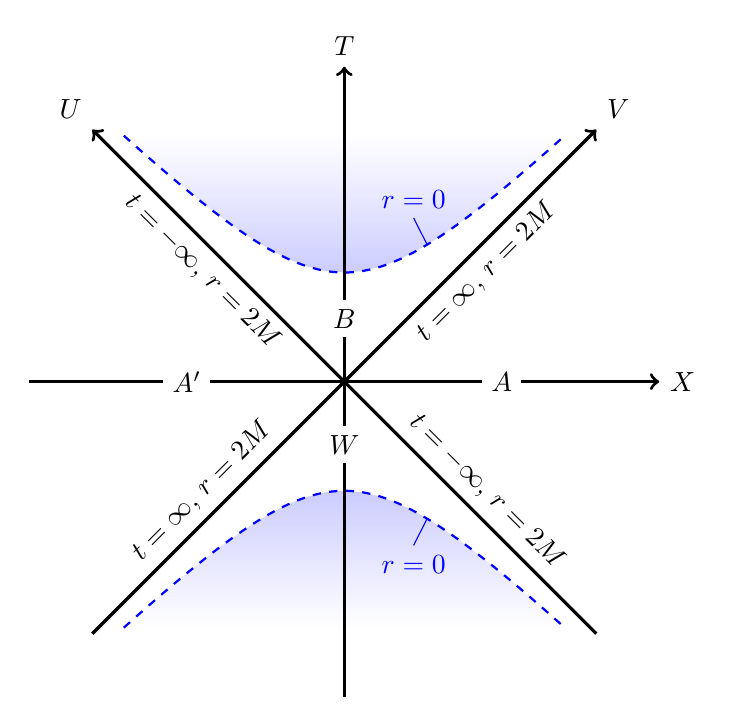
\begin{tikzpicture}[scale=0.8]
	% 蓝色阴影, 渐变
	\shade [top color=white, bottom color=blue!20, domain=-3.5:3.5, variable=\X] plot ({\X}, {sqrt(\X*\X+3)}) -- cycle;
	% 粗虚线
	\draw [blue, dashed, thick, domain=-3.5:3.5, smooth, variable=\X] plot (\X,{sqrt(\X*\X+3)});
	% r=0 标识
	\draw [blue] (1.315,{sqrt(4.73)}) -- (1.1,2.6) node [above] {$r=0$};
	% 下半部分的粗虚线和 r=0 标识
	\shade [top color=blue!20, bottom color=white, domain=-3.5:3.5, variable=\X] plot ({\X}, {-sqrt(\X*\X+3)}) -- cycle;
	\draw [blue, dashed, thick, domain=-3.5:3.5, smooth, variable=\X] plot (\X,{-sqrt(\X*\X+3)});
	\draw [blue] (1.315,{-sqrt(4.73)}) -- (1.1,-2.6) node [below] {$r=0$};
	% 绘制 (X,T) 坐标轴, 非常粗, 单向箭头
	\draw [very thick, ->] (-5,0) -- (0,0) node [midway,fill=white] {$A'$} -- (5,0) node [midway,fill=white] {$A$} node [right] {$X$}; 
	\draw [very thick, ->] (0,-5) -- (0,0) node [pos=.8,fill=white] {$W$} -- (0,5) node [pos=.2,fill=white] {$B$} node [above] {$T$};
	% 绘制斜向坐标轴
	\draw [very thick, ->] (-4,-4) -- (0,0) node [sloped, midway, above]  {$t=\infty,\,r=2M$} -- (4,4) node [sloped, midway, below]  {$t=\infty,\,r=2M$} node [above right] {$V$};
	\draw [very thick, ->] (4,-4) -- (0,0) node [sloped, midway, above]  {$t=-\infty,\,r=2M$} -- (-4,4) node [sloped, midway, below]  {$t=-\infty,\,r=2M$}  node [above left] {$U$};
\end{tikzpicture}
\caption{Kruskal 延拓\hspace{2em}}
\label{Kruskal1}
\end{figure}

注意, 目前看来 图 \ref{Kruskal1} 中的 $A'$ 和 $W$ 只是数学上的结果, 现实中黑洞是否真的连接两个宇宙, 白洞是否真的存在还需另作讨论. 图 \ref{Kruskal1} 中只有 $A$ 区、$B$ 区、$V$ 的正半轴具有物理意义. 

我们还可以进一步画出 $Kruskal$ 延拓中的等 $t$ 面和等 $r$ 面来帮助理解.

\begin{figure}[H]
\centering
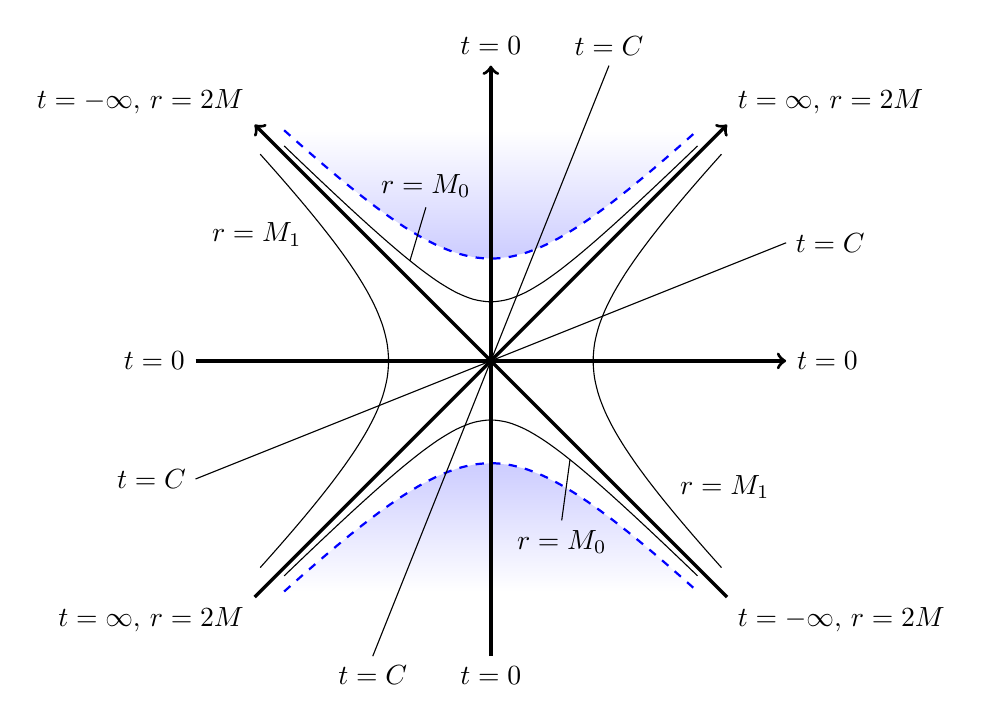
\begin{tikzpicture}[scale=0.75]
	% 蓝色阴影, 渐变, 边界绘制粗虚线.
	\shade [top color=white, bottom color=blue!20, domain=-3.5:3.5, variable=\X] plot ({\X}, {sqrt(\X*\X+3)}) -- cycle;
	\draw [blue, dashed, thick, domain=-3.5:3.5, smooth, variable=\X] plot (\X,{sqrt(\X*\X+3)});
	\shade [top color=blue!20, bottom color=white, domain=-3.5:3.5, variable=\X] plot ({\X}, {-sqrt(\X*\X+3)}) -- cycle;
	\draw [blue, dashed, thick, domain=-3.5:3.5, smooth, variable=\X] plot (\X,{-sqrt(\X*\X+3)});
	% 等 r 面
	\draw [-, domain=-3.5:3.5, smooth, variable=\X] plot (\X,{sqrt(\X*\X+1)});
	\draw (-1.37,{sqrt(2.8769)}) -- (-1.1,2.6) node [above] {$r=M_0$};
	\draw [-, domain=-3.5:3.5, smooth, variable=\X] plot (\X,{-sqrt(\X*\X+1)});
	\draw (1.34,{-sqrt(2.7956)}) -- (1.2,-2.7) node [below] {$r=M_0$};
	\draw [-, domain=-3.5:3.5, smooth, variable=\X] plot ({sqrt(\X*\X+3)},\X);
	\draw ({sqrt(9.25)},-2.5) node [above right] {$r=M_1$};
	\draw [-, domain=-3.5:3.5, smooth, variable=\X] plot ({-sqrt(\X*\X+3)},\X);
	\draw ({-sqrt(9.25)},2.5) node [below left] {$r=M_1$};
	% 坐标轴
	\draw [very thick, ->] (-5,0) node[left]{$t=0$} -- (5,0) node[right]{$t=0$}; 
	\draw [very thick, ->] (0,-5) node[below]{$t=0$} -- (0,5) node[above]{$t=0$};
	\draw [very thick, ->] (-4,-4) node [below left] {$t=\infty,\,r=2M$} -- (4,4) node [above right] {$t=\infty,\,r=2M$};
	\draw [very thick, ->] (4,-4) node [below right] {$t=-\infty,\,r=2M$} -- (-4,4) node [above left] {$t=-\infty,\,r=2M$};
	% 等 t 面
	\draw [-] (-5,-2) node [left] {$t=C$} -- (5,2) node [right] {$t=C$};
	\draw [-] (-2,-5) node [below] {$t=C$} -- (2,5) node [above] {$t=C$};
\end{tikzpicture}
\caption{Kruskal 延拓中的等 $t$ 面和等 $r$ 面, 其中 $C>0$, $0<M_0<2M$, $M_1>2M$}
\label{Kruskal2}
\end{figure}

\begin{figure}[H]
\centering
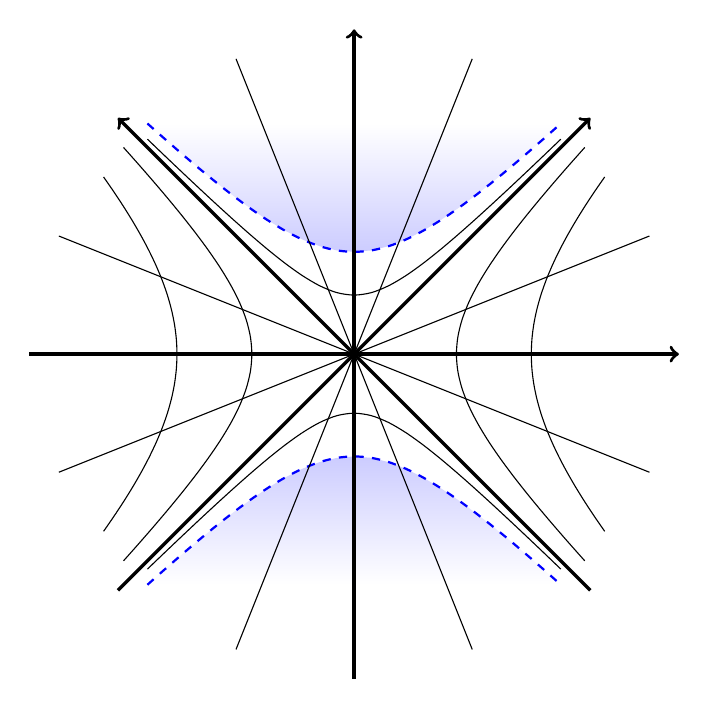
\begin{tikzpicture}[scale=0.75]
	% 蓝色阴影, 渐变, 边界绘制粗虚线.
	\shade [top color=white, bottom color=blue!20, domain=-3.5:3.5, variable=\X] plot ({\X}, {sqrt(\X*\X+3)}) -- cycle;
	\draw [blue, dashed, thick, domain=-3.5:3.5, smooth, variable=\X] plot (\X,{sqrt(\X*\X+3)});
	\shade [top color=blue!20, bottom color=white, domain=-3.5:3.5, variable=\X] plot ({\X}, {-sqrt(\X*\X+3)}) -- cycle;
	\draw [blue, dashed, thick, domain=-3.5:3.5, smooth, variable=\X] plot (\X,{-sqrt(\X*\X+3)});
	% 等 r 面
	\draw [-, domain=-3.5:3.5, smooth, variable=\X] plot (\X,{sqrt(\X*\X+1)});
	\draw [-, domain=-3.5:3.5, smooth, variable=\X] plot (\X,{-sqrt(\X*\X+1)});
	\draw [-, domain=-3.5:3.5, smooth, variable=\X] plot ({sqrt(\X*\X+3)},\X);
	\draw [-, domain=-3.5:3.5, smooth, variable=\X] plot ({-sqrt(\X*\X+3)},\X);
	\draw [-, domain=-3:3, smooth, variable=\X] plot ({sqrt(\X*\X+9)},\X);
	\draw [-, domain=-3:3, smooth, variable=\X] plot ({-sqrt(\X*\X+9)},\X);
	% 坐标轴
	\draw [very thick, ->] (-5.5,0) -- (5.5,0); 
	\draw [very thick, ->] (0,-5.5)-- (0,5.5);
	\draw [very thick, ->] (-4,-4) -- (4,4);
	\draw [very thick, ->] (4,-4)-- (-4,4);
	% 等 t 面
	\draw [-] (-5,-2) -- (5,2);
	\draw [-] (-5,2) -- (5,-2);
	\draw [-] (-2,-5) -- (2,5);
	\draw [-] (2,-5) -- (-2,5);
\end{tikzpicture}
\caption{Kruskal 延拓中的等 $t$ 面和等 $r$ 面构成的网格}
\label{Kruskal3}
\end{figure}

\subsection{史瓦西黑洞}
\label{black hole}
至此, 我们解出了真空爱因斯坦场方程的一个解, 并对其进行了延拓. 但我们还没有解释为什么史瓦西度量可以被用来描述黑洞, $r=2M$ 又为什么叫做事件视界. 为了进一步解释史瓦西度量的物理含义, 我们介绍一个重要结论.
\begin{theorem}[Birkhoff 定理{\cite{hawking2023large}}]
\label{Birkhoff}
	真空爱因斯坦场方程的球对称解一定是史瓦西度量.
\end{theorem}

Birkhoff 定理说明史瓦西度量确实描述的是质量为 $M$ 的小球所产生的引力场 (小球无自转且不带电). 恒星通过内部的核聚变释放能量来对抗引力, 在恒星演化的末期, 引力胜于聚变, 于是恒星会进行{\bf 引力坍缩}(gravitational collapse), 引力坍缩有以下几种结局:
\begin{enumerate}
	\item 引力坍缩导致恒星密度增大, 进而导致{\bf 电子简并压}(electron degenerate pressure)增大, 若电子简并压足以抗衡引力, 则会形成{\bf 白矮星}(white dwarf).
	\item 若电子简并压不足以抗衡引力, 恒星会进一步坍缩, 坍缩导致周围环境非常极端, 以至于恒星的成分基本都变成了中子, 这时恒星会进行{\bf 超新星爆发} (supernova explosion).此时若{\bf 中子简并压}足以抗衡引力, 则会形成{\bf 中子星}(neutron star).
	\item 若中子简并压也无法抗衡引力, 则恒星会进一步坍缩形成{\bf 黑洞}.
\end{enumerate}

为了进一步讨论史瓦西黑洞, 我们定义
\[ v:=t+r_*, \] 
其中 $r_*$ 为乌龟坐标, 坐标系 $\{v,r,\theta,\varphi\}$ 叫做Eddington-Finkelstein 坐标系. 由于
\begin{align*}
	&\phantom{{}={}}-\left( 1-\frac{2M}{r} \right)\mathrm{d}v^2+2\,\mathrm{d}v \mathrm{d}r\\
	&=-\left( 1-\frac{2M}{r} \right)(\mathrm{d}t^2+2\,\mathrm{d}t\mathrm{d}r_*+\mathrm{d}r_*^2)+2(\mathrm{d}t\mathrm{d}r+\mathrm{d}r_*\mathrm{d}r)\\
	&= -\left(1-\frac{2M}{r}\right)\mathrm{d}t^2+\left( 1-\frac{2M}{r} \right)^{-1}\mathrm{d}r^2,
\end{align*}
注意到上式第一行只有一个奇点 $r=0$, 因此也可以在这个坐标系下对史瓦西度量进行延拓. 延拓后, $\{v,r\}$ 可以覆盖图 \ref{Kruskal1} 中的 $A$ 区和$B$ 区以及 $V$ 的正半轴, 这已足够用来讨论史瓦西黑洞了.

\begin{remark}
	这样定义的 $v$ 也同样出现在 Kruskal 延拓的过程中.
\end{remark}

若一条曲线的参数表达式 $(v(\lambda),r(\lambda),\theta(\lambda),\varphi(\lambda))$ 中后两项均为常值, 则称其为径向曲线. 对于任意径向类光曲线, 设其参数表达式为 $(v(\lambda),r(\lambda))$, 则
\begin{align*}
	0 &= -\left( 1-\frac{2M}{r} \right)\left( \frac{\mathrm{d} v}{\mathrm{d} \lambda} \right)^2+2\frac{\mathrm{d} v}{\mathrm{d} \lambda}\frac{\mathrm{d} r}{\mathrm{d} \lambda}=\left[ -\left( 1-\frac{2M}{r} \right)\frac{\mathrm{d} v}{\mathrm{d} \lambda}+2\frac{\mathrm{d} r}{\mathrm{d} \lambda} \right]\frac{\mathrm{d} v}{\mathrm{d} \lambda}.
\end{align*}
解上述方程, 首先显然 $r=2M$ 是一个解, 然后
\begin{align*}
	r\neq 2M,\ \frac{\mathrm{d} v}{\mathrm{d} \lambda}\neq 0&\implies \frac{\mathrm{d} v}{\mathrm{d} r}=\frac{2r}{r-2M}\\
	&\implies v=4M\log|r-2M|+2r+C,\\
	\frac{\mathrm{d} v}{\mathrm{d} \lambda}= 0&\implies v=C.
\end{align*}
我们接下来要把这两族类光曲线画出来, 但 $v=C$ 在 $\{v,r\}$ 中是水平直线, 不够直观, 于是我们定义
\[ \tilde{t}:=v-r, \] 
并在 $\{\tilde{t},r\}$ 坐标系中将类光曲线画出来.
\begin{figure}[H]
\centering
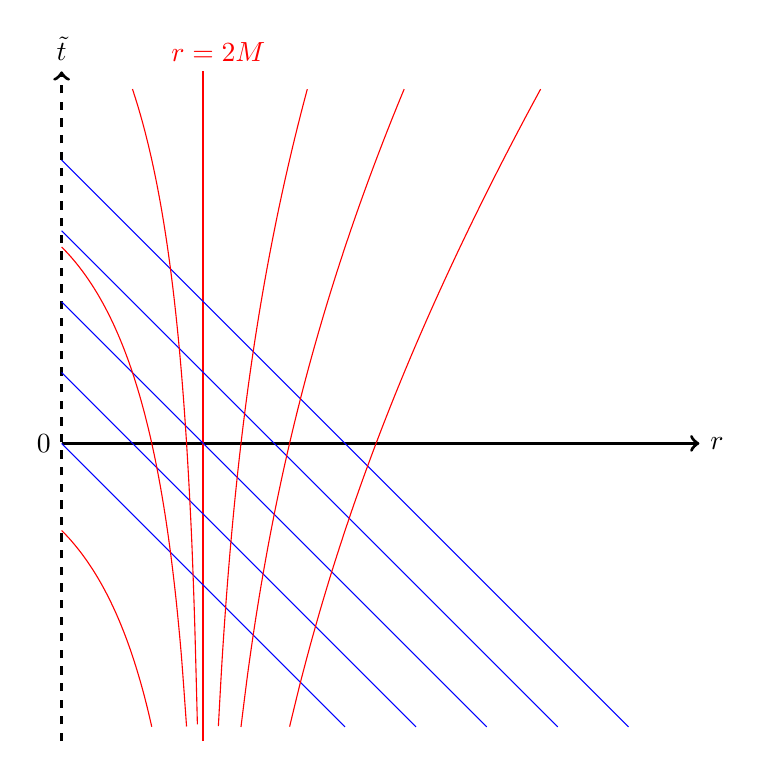
\begin{tikzpicture}[scale=0.9]
	% 坐标轴
	\draw [very thick, ->] (0,0) -- (9,0) node [right] {$r$}; 
	\draw [dashed, very thick, ->] (0,-4.2) -- (0,0) node [left] {$0$} -- (0,5.25) node [black, above] {$\tilde{t}$};
	% 事件视界
	\draw [red, thick, -] (2,-4.2) -- (2,5.25) node [above] {$\phantom{M}r=2M$};
	% 类光曲线
	\draw [blue, -] (0,4) -- (8,-4);
	\draw [blue, -] (0,3) -- (7,-4);
	\draw [blue, -] (0,2) -- (6,-4);
	\draw [blue, -] (0,1) -- (5,-4);
	\draw [blue, -] (0,0) -- (4,-4);
	
	\draw [red, domain=2.212:3.467, smooth, variable=\r] plot (\r,{4*ln(\r-2)+\r});
	\draw [red, domain=2.531:4.834, smooth, variable=\r] plot (\r,{4*ln(\r-2)+\r-4});
	\draw [red, domain=3.217:6.759, smooth, variable=\r] plot (\r,{4*ln(\r-2)+\r-8});
	\draw [red, domain=0:1.763, smooth, variable=\r] plot (\r,{4*ln(2-\r)+\r});
	\draw [red, domain=0:1.272, smooth, variable=\r] plot (\r,{4*ln(2-\r)+\r-4});
	\draw [red, domain=1:1.916, smooth, variable=\r] plot (\r,{4*ln(2-\r)+\r+4});
\end{tikzpicture}
\caption{$\{\tilde{t},r\}$ 坐标系中的类光曲线}
\label{t-r}
\end{figure}
\begin{remark}
	$-\infty<\tilde{t}<+\infty$, $0<r<+\infty$.
\end{remark}

通过观察图 \ref{t-r}, 我们发现 $r=2M$ 本身是一条类光曲线, 以它为分界, 事件视界以内的光子只能朝着 $r=0$ 行进, 而事件视界以外的光子则不受这种限制. 

\begin{definition}[光锥]
	对于时空中的一点 $p$, 我们称所有过点 $p$ 的类时曲线与类光曲线的并为点 $p$ 处的{\bf 光锥}(light cone).
\end{definition}

点 $p$ 处的光锥就是时空中所有可以与点 $p$ 产生因果联系的部分, 图 \ref{light cone} 展示了 $\{\tilde{t},r\}$ 坐标系中一些点处的 (局部) 光锥.
\begin{figure}[H]
\centering
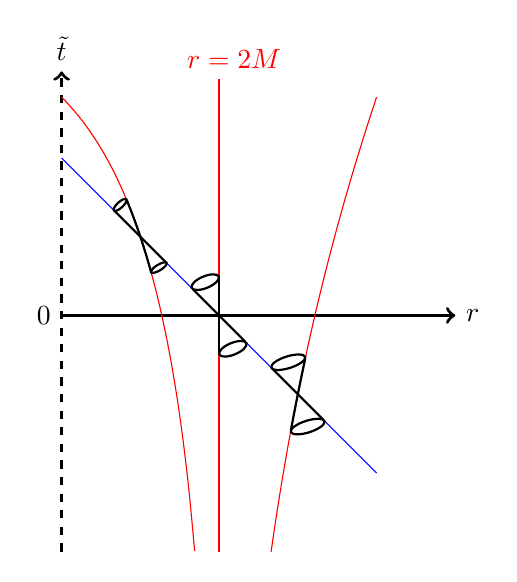
\begin{tikzpicture}[scale=1]
	% 坐标轴
	\draw [very thick, ->] (0,0) -- (5,0) node [right] {$r$}; 
	\draw [dashed, very thick, ->] (0,-3) -- (0,0) node [left] {$0$} -- (0,3.1) node [black, above] {$\tilde{t}$};
	% 事件视界
	\draw [red, thick, -] (2,-3) -- (2,3) node [above] {$\phantom{M}r=2M$};
	% 类光曲线
	\draw [blue, -] (0,2) -- (4,-2);
	\draw [red, domain=2.660:4, smooth, variable=\r] plot (\r,{4*ln(\r-2)+\r-4});
	\draw [red, domain=0:1.69, smooth, variable=\r] plot (\r,{4*ln(2-\r)+\r});
	% 光锥
	\draw [thick] (1.666,0.334) -- (2.334,-0.334);
	\draw [thick] (2,-0.471) -- (2,0.471);
	\draw [thick] (1.824,0.423) circle [x radius = 0.186, y radius = 0.075, rotate = 22.5];
	\draw [thick] (2.175,-0.423) circle [x radius = 0.186, y radius = 0.075, rotate = 22.5];
	\draw [thick] (2.67,-0.67) -- (3.329,-1.329);
	\draw [thick, domain=2.911:3.095, smooth, variable=\r] plot (\r,{4*ln(\r-2)+\r-4});
	\draw [thick] (2.878,-0.594) circle [x radius = 0.225, y radius = 0.075, rotate = 17.43];
	\draw [thick] (3.125,-1.411) circle [x radius = 0.224, y radius = 0.075, rotate = 17.7];
	\draw [thick] (0.667,1.333) -- (1.333,0.667);
	\draw [thick, domain=0.825:1.137, smooth, variable=\r] plot (\r,{4*ln(2-\r)+\r}); 
	\draw [thick] (0.743,1.404) circle [x radius = 0.106, y radius = 0.037, rotate = 42.3];
	\draw [thick] (1.235,0.608) circle [x radius = 0.115, y radius = 0.037, rotate = 31.26];
\end{tikzpicture}
\caption{$\{\tilde{t},r\}$ 坐标系中的光锥}
\label{light cone}
\end{figure}
通过观察图 \ref{light cone}, 我们发现只能质点满足 $r\leq 2M$, 它就只能朝着 $r=0$ 运动. 因此只要恒星的半径坍缩至 $r=2M$, 它就只能继续一路坍缩下去, 且会在有限时间内缩为一个点 $r=0$, 也就是说史瓦西黑洞的全部质量都集中在一点, 此时史瓦西度量适用于除 $r=0$ 外的整个时空.
\begin{remark}
	这就是 $r=0$ 叫做时空奇点或引力奇点的原因.
\end{remark}

另外, 对于事件视界内的一点, 其指向未来的光锥完全包含于视界之内, 因此视界内发生的任何事都不会对视界外产生影响, 视界内的任何信息都无法传达到视界外.

\begin{remark}
	这就是 $r=2M$ 叫做事件视界的原因.
\end{remark}

通过分析 $\{\tilde{t},r\}$ 坐标系中的类光曲线, 我们可以预想: 若一位探险者勇敢地跳入黑洞, 在穿越视界时, 它不会有什么特殊的感觉; 但在视界外的人看来, 它靠近视界的速率越来越慢, 直到永远.

\begin{remark}
	且在外界的人看来, 探险者发出的电磁波红移程度也越来越大, 因此 $r=2M$ 也叫做{\bf 无限红移面} \cite[\S\,9.4.4]{梁灿彬2000微分几何入门与广义相对论}. 类似地, 视界外部的人也可以永远收到恒星坍缩成黑洞前的瞬间所发出的电磁波, 且红移程度越来越大.
\end{remark}

\subsection{黑洞无毛}
对于质量为 $M$, 电荷量为 $Q$, 无自转的球形天体, 其外部的时空中的度量为
\[ \mathrm{d}s^2=-\left( 1-\frac{2M}{r}+\frac{Q^2}{r^2} \right)\mathrm{d}t^2+\left( 1-\frac{2M}{r}+\frac{Q^2}{r^2} \right)^{-1}\mathrm{d}r^2+r^2(\mathrm{d}\theta^2+\sin^2\theta\,\mathrm{d}\varphi^2). \] 
这个度量叫做 {\bf Reissner-Nordstrom 度量} (RN 度量), 当 $Q=0$ 时它会退化为史瓦西度量, 详见 \cite[\S\,8.4]{梁灿彬2000微分几何入门与广义相对论}. 与史瓦西度量类似, RN 度量可以用来描述会自转的黑洞, 详见 \cite[\S\,13.1]{梁灿彬2000微分几何入门与广义相对论}; 且爱因斯坦-麦克斯韦方程 (即麦克斯韦场方程与麦克斯韦方程的联合) 的任一渐近平直的球对称解一定是 RN 度量.

对于质量为 $M$, 电荷量为 $Q$, 绕 $\theta=0$ 旋转的球形天体, 记其角动量的大小为 $J$, 并记单位质量对应的角动量为 $a:=J/M$, 则其外部的时空中的度量为
\begin{align*}
	\mathrm{d}s^2 &=-\left[ 1-\frac{2Mr-Q^2}{\rho^2} \right]\mathrm{d}t^2+\frac{\rho^2}{\Delta}\,\mathrm{d}d^2+\rho^2\,\mathrm{d}\theta^2\\
	&\phantom{{}={}}+\left[ (a^2+r^2)^2-\Delta a^2\sin^2\theta \right]\frac{\sin^2\theta}{\rho^2}\,\mathrm{d}\varphi^2\\
	&\phantom{{}={}}-(2Mr-Q^2)\frac{2a\sin^2\theta}{\rho^2}\,\mathrm{d}t\mathrm{d}\varphi,
\end{align*} 
其中 
\begin{align*}
	\rho^2&=r^2+a^2\cos^2\theta,\\
	\Delta&=r^2-2Mr+a^2+Q^2.
\end{align*}
这个度量叫做 {\bf Kerr-Newman 度量} (KN 度量), 当 $a=0$ 时它会退化为 RN 度量, 当 $a=Q=0$ 时, 它会退化为史瓦西度量. 另外, 当 $Q=0$ 时所得到的度量叫做 {\bf Kerr 度量}, 它对应自转但不带电的球形天体. 与前面提到的度量类似, KN 度量可以用来描述带电黑洞, 详见 \cite[第 13 章]{梁灿彬2000微分几何入门与广义相对论}.

关于上面提到的几种黑洞, 有如下唯一性定理 \cite[\S\,13.6]{梁灿彬2000微分几何入门与广义相对论}:
\begin{enumerate}
	\item 真空爱因斯坦方程的静态黑洞解必为史瓦西度量.
	\item 爱因斯坦-麦克斯韦方程的静态黑洞解必为 RN 度量.
	\item 爱因斯坦-麦克斯韦方程的稳态轴对称黑洞解必为 KN 度量.
\end{enumerate}
\begin{remark}
	这里的静态和稳态指的是在事件视界外的静态和稳态.
\end{remark}
基于这三个定理, Wheeler 于 $1971$ 年提出了{\bf 黑洞无毛猜想}(no-hair conjecture).
\begin{definition}[黑洞无毛猜想]
	稳态黑洞由三个外部可观测量 $M,J,Q$ 唯一决定.
\end{definition}